\section{Introduction}
A major reason for the incredible diversity of Arthropoda is their successful colonization of terrestrial environments and their ability to adapt to the environmental extremes found there. We will discuss hypotheses and evidence concerning the emergence of arthropods from marine habitats. What did early arthropods look like, and what challenges did they face? How are fossils formed, and what kinds of information can we derive from them (and what \textit{can't} we get from them)? Where do we find fossils? 

\section{Taphonomy}
\latinword{Taphonomy} is the study of how organisms decay after dying, how they settle into positions that may result in fossilization, and how those fossils change chemically, geologically, \textit{etc}. over time. In this lab we have demonstrations that represent two elements of taphonomy: \latinword{decomposition}, the decay of a carcass, and \latinword{biostratinomy}, the processes that affect a carcass prior to deposition. The intention is to get you thinking about biases in the fossil record. The geologic elements of taphonomy, diagenesis for example, are beyond the scope of this class.

\subsection{Insects trapped in resin}
Amber is fossilized tree resin---\textit{i.e.}, the viscous compounds produced by plants, in response to damage. One can imagine that oozing, sticky goo from tree wounds would be a prime attractant for (some) insects. Many insects get trapped, and, if the conditions are right, their fates are preserved for us to see, millions of years later. We'll look at some real amber fossils, but first we'll try an experiment.

\begin{theo}
{}Jot down a few biases you would expect to see in amber fossils. Think about the insect morphology and natural history. Are there certain behaviors or structures that lend themselves to entrapment or escape? Why would an insect be attracted to resin? Or would they?\end{theo}\vspace{3mm}

\noindent{}We've provided several insect specimens and parts. Using your forceps, try sticking these specimens, one at a time, in a drop of Canada balsam. Does it stick?

\begin{theo}
{}What difference, if any, do you see in the way that specimens interact with this sticky substrate. Given these observations, what would you expect to see in the fossil record and why?\end{theo}\vspace{3mm}

\subsection{Insects decomposing}
Most non-amber fossils (compression fossils, concretions, ichnofossils, \textit{etc}.) are derived from insects that became trapped or otherwise interacted with aquatic and/or sedimentary environments. Several specimens have been placed in situations that simulate early taphonomy of these fossils. Take some time predict and observe the condition of each before answering the next question.\vspace{3mm}

\begin{theo}
{}Describe what you see in each jar. Based on their decomposition, what would you predict about the fossil record and potential biases?\end{theo}

\section{Fossil arthropods}
Our collection holds several arthropod fossils, each from a different \latinword{Lagerst\"atte}: 

\paragraph{Ichnofossil, unknown source (probably Carboniferous, $\sim$359--299 Mya)} This greenish, flat sedimentary rock has multiple track ways across it.

\paragraph{Old Port Formation, Shriver member (Early Devonian, $\sim$419--393 Mya)} These sedimentary rocks, which were collected in Huntingdon Co., Pennsylvania, are dark gray or orange-yellow in color, with molds and fossils of trilobites. These arthropods lived in the ocean, which covered much of Pennsylvania in the Devonian. Be sure to find the fossil that includes a trilobite's compound eye.

\paragraph{Creede Formation (Oligocene, $\sim$27 Mya)} You will see several grayish, flat rocks that have compression fossils in them, similar to figure \ref{fig:creedeFossil}. These insects lived in and around a shallow, high altitude lake in what is now Creede, CO. The lake was repeatedly filled with volcanic ash, from eruptions and from runoff \citep{berkeley}.

\begin{figure}[ht!]
  \centering
    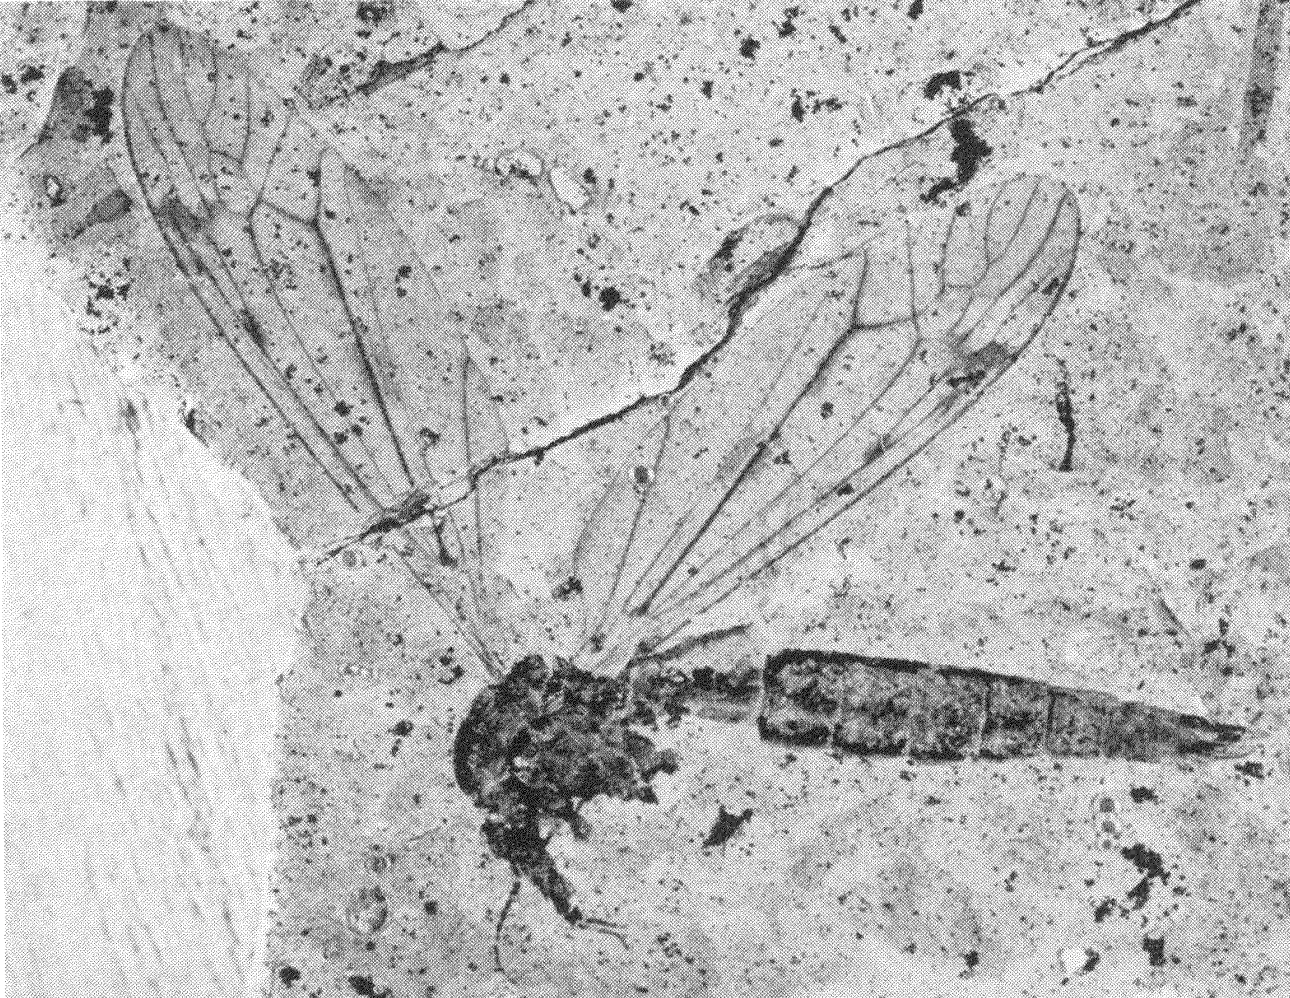
\includegraphics[width=0.35\textwidth]{creedeFossil}
  \caption{Crane fly, Creede Formation. \citep[][Fig. 1]{carpenter1938fossil}}
  \label{fig:creedeFossil}
\end{figure}

\paragraph{Dominican amber (Middle Miocene, 15--20 Mya)} We have a small collection of amber with insect inclusions. These insects lived in what is now the Dominican Republic. This amber is the fossilized resin from a leguminous tree, \textit{Hymenaea protera} (Fabaceae), now extinct \citep{IturraldeVinent1850}.

\paragraph{Barstow Formation (Early to Middle Miocene, 19.3--13.4 Mya)} These fossils are quite small and are mounted on slides. These insects are presumed to have lived in a series of saline-alkaline lakes that was repeatedly subjected to volcanic disturbance. Eruptions repeatedly killed the lakes' fauna and covered the carcasses with ash and calcium carbonate. The subsequent chemistry allowed silica to replace the integument and for the preservation of soft tissues \citep{PARK01042001}.

\begin{theo}
{}Spend some time with each type of fossil. Are they biased towards some particular life history or body part, as you hypothesized in section 1? Sketch a couple specimens in your lab notebook and label the parts. Which fossils offer the most information and why? How did the trilobite's compound eye get preserved? What can you infer from the trackways?\end{theo}

\section{Terrestrial adaptations}
We discussed the terrestrialization of Arthropoda and Earth's early history. Take a few minutes to remind yourself of the challenges faced by marine organisms as they moved onto land, before moving on to the next two demonstrations.

\subsection{Respiration}
In the morphology lab you learned about spiracles and tracheae, the primary mechanism through which most terrestrial hexapods respire. Think about how these structures are adapted for an environment that threatens desiccation. Now examine a decapod and a xiphosuran (horseshoe crab) and see if you can identify the structures associated with respiration. Can you find analogous structures on a terrestrial isopod, a scorpion, or a spider? What about an onychophoran?

\subsection{Integument}
Let's take a quick look at some other adaptions to terrestrial, and in this case very, very dry habitats. Death-feigning beetles (Tenebrionidae: \textit{Asbolus verrucosus} (LeConte, 1852)) live in the Sonoran Desert. Gently pick one up and look at it under the microscope.

\begin{theo}
{}Sketch the respiratory structures you can find in the decapod, the terrestrial isopod, the xiphosuran, and the scorpion. How do the terrestrial taxa remediate water loss? Can you see any relevant traits in the death-feigning beetle?\end{theo}

\section*{Test yourself}
Before moving on make sure you're comfortable with the following concepts. Could you write a couple sentences that explain each term? Can you provide examples?

\begin{enumerate} 
\item{\textit{Lagerst{\"a}tte}} 
\item{taphonomy}  
\item {stem \textit{vs}. crown group}
\end{enumerate}

\noindent{}Can you describe three types of fossils and how they occur? What factors influence preservation, and what environmental conditions result in well-preserved fossils? \citep[Hint: see][]{taphonomy2004}\vspace{3mm}

\noindent{Given what we know about insect bodies and biology, what biases would you expect to see in the fossil record and why?}\vspace{3mm}

\noindent{What can fossils tell us about insect evolution and biology?}\vspace{3mm}

\noindent{When did arthropods originate and in what environmental context? What about Insecta?}\vspace{3mm}

\noindent{We discussed the evolution of Arthropods through nine geologic periods, beginning with the Cambrian. Can you name these periods and describe in one to three sentences the relevance of each---environmental conditions (generally), types of insects present, and where to find fossils?}\vspace{3mm}

\noindent{What characteristics of the arthropod \textit{Bauplan} allowed these organisms to move into terrestrial environments? When and how many times (minimally) did this happen?

\clearpage
\thispagestyle{empty}
